\chapter{Utilizarea aplicației și funcționalități}

\section{Prezentarea interfeței}

Ruta implictă, la accesarea aplicației, este „/login”. În figurile \ref{fig:taskage-login}\ și \ref{fig:taskage-login-auto} este prezentată interfața încărcată ca răspuns, în cele două contexte posibile: autentificare explicită și autentificare automată. Aceste pagini sunt rezultatul procesului complex care se declanșează la accesarea rutei „/login”, proces descris în secțiunea 4.1.

În cazul în care browser-ul nu conține în local storage un token de autentificare, sau token-ul găsit este expirat, este afișat un formular de autentificare. Aici, utilizatorul trebuie să introducă credențialele primite de la administrator, singurul tip de utilizator care are privilegiul creării conturilor. Datele sunt preluate din formular și trimise către componenta Taskage-Core, iar răspunsul este transformat într-un toast explicit cu feedback legat de succesul acțiunii. 

 \begin{figure}[H]
	\centering
 	 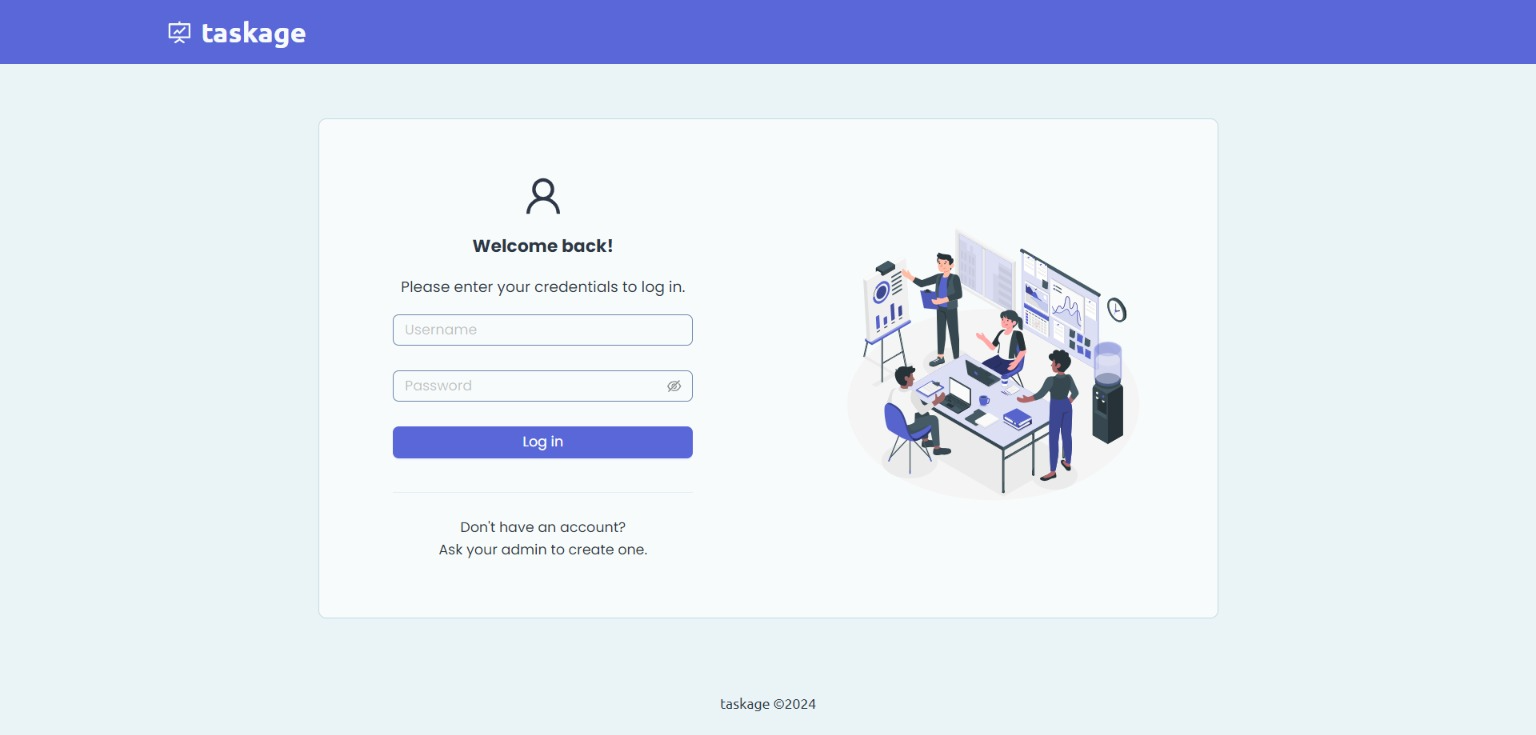
\includegraphics[width=\linewidth]{taskage-login.png}
	\caption{Pagina încărcată de ruta „/login” fără autentificare automată}
	\label{fig:taskage-login}
 \end{figure}

Ca urmare a autentificării explicite, în proprietatea localStorage a browser-ului se salvează un obiect numit „authenticated-user”, care conține atât datele utilizatorului cât și token-ul de acces al acestuia(figura \ref{fig:taskage-login-auto}).

 \begin{figure}[H]
	\centering
 	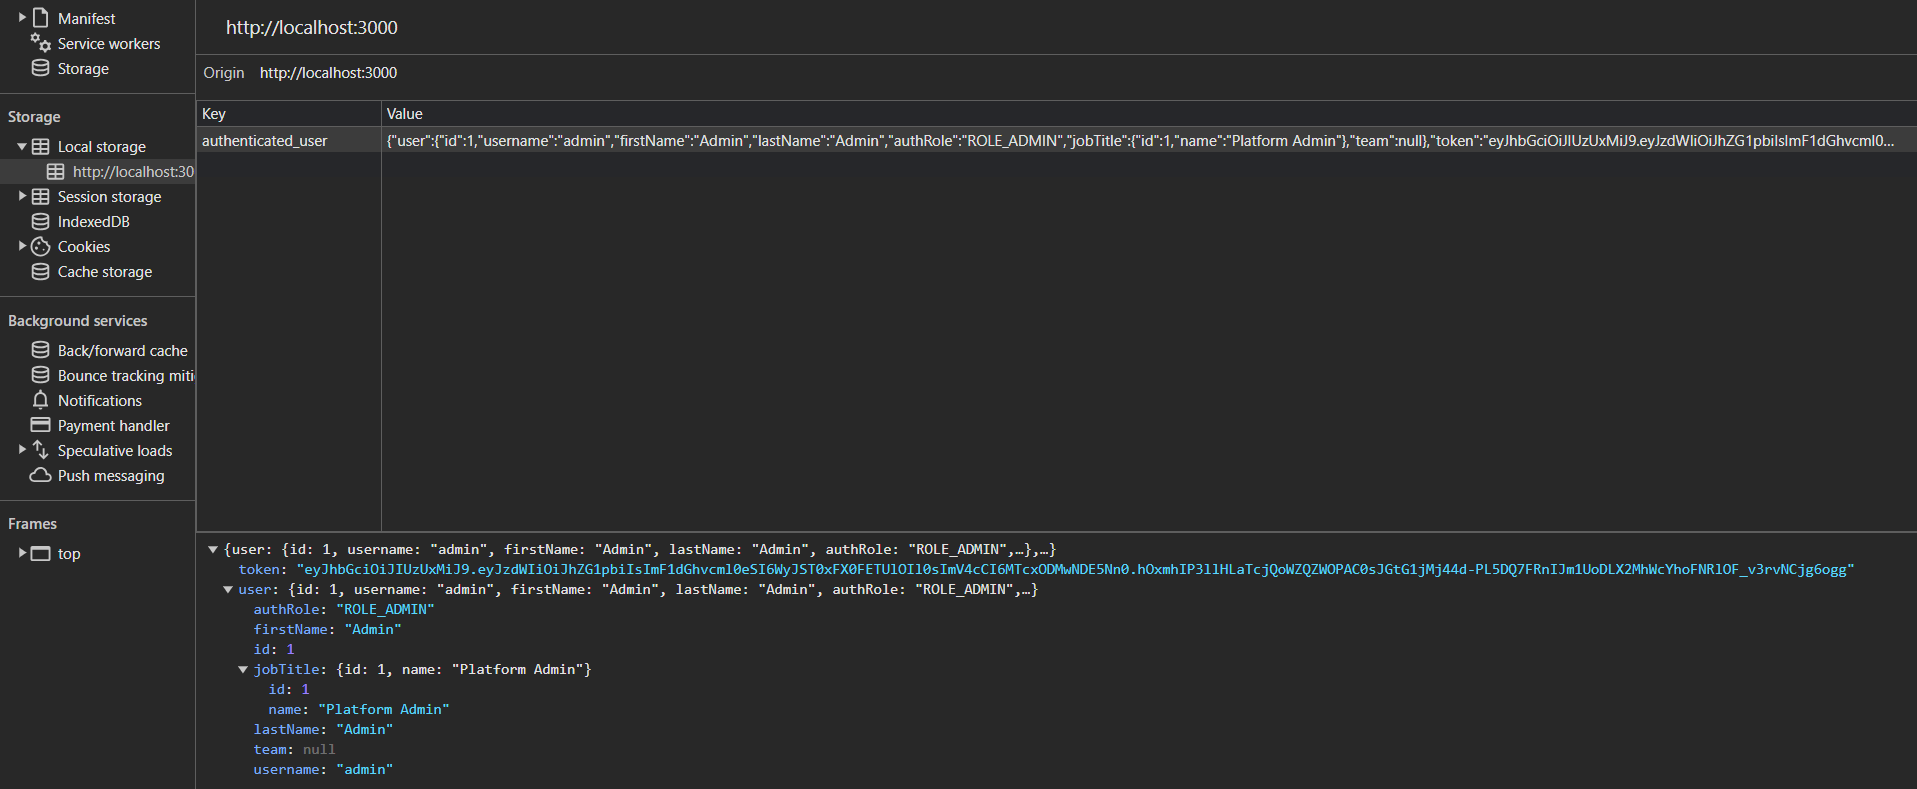
\includegraphics[width=\linewidth]{localstorage-token.png}
	\caption{Obiectul salvat în localStorage după autentificare}
	\label{fig:token}
 \end{figure}

Atunci când browser-ul conține în localStorage un token care nu a expirat, se realizează autentificarea automată, iar utilizatorul este redirecționat către propriul panou de control și primește un toast sugestiv, așa cum apare în a doua captură de ecran(figura \ref{fig:taskage-login-auto}). De asemenea, acesta este anunțat printr-o notificare de faptul că autentificarea s-a realizat automat și poate să se deconecteze explicit prin butonul „Log Out”, prezent în header.

 \begin{figure}[H]
	\centering
 	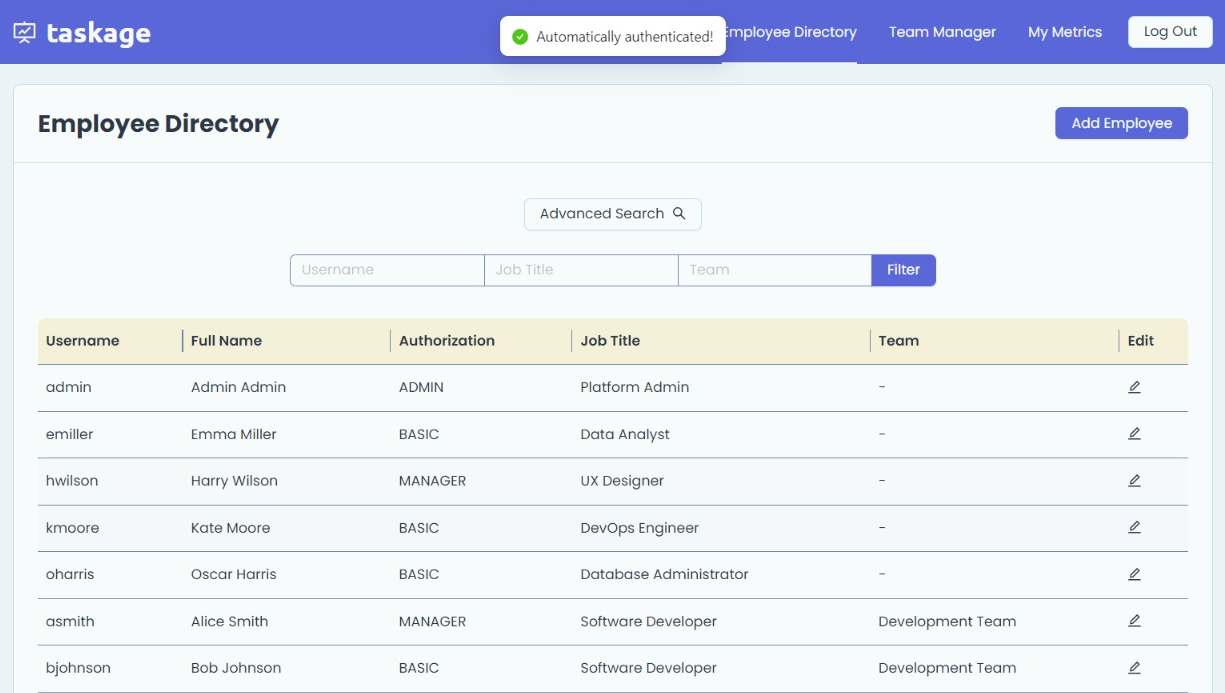
\includegraphics[width=\linewidth]{taskage-login-redirect-1.png}
	\caption{Pagina răspuns în urma autentificării automate}
	\label{fig:taskage-login-auto}
 \end{figure}

Paleta de culori este setată asupra componentelor Ant Design prin intermediul componentei „ConfigProvider”, care pune la dispoziție prop-ul „theme”. Aici, tema de culori poate fi indicată prin cheia „components”, care aplică stilul pe componente specifice ale bibliotecii, sau „tokens”, care aplică stilul prin etichetele indicați în documentație ca fiind asociate anumitor componente.

Mai departe, fluxul utilizării aplicației depinde de tipul de utilizator(BASIC, MANAGER sau ADMIN) care s-a autentificat, diferențiere făcută prin token-ul de autorizare, generat anterior, acum trimis ca Authorization header pentru fiecare request(figura \ref{fig:auth-token}).

 \begin{figure}[H]
	\centering
 	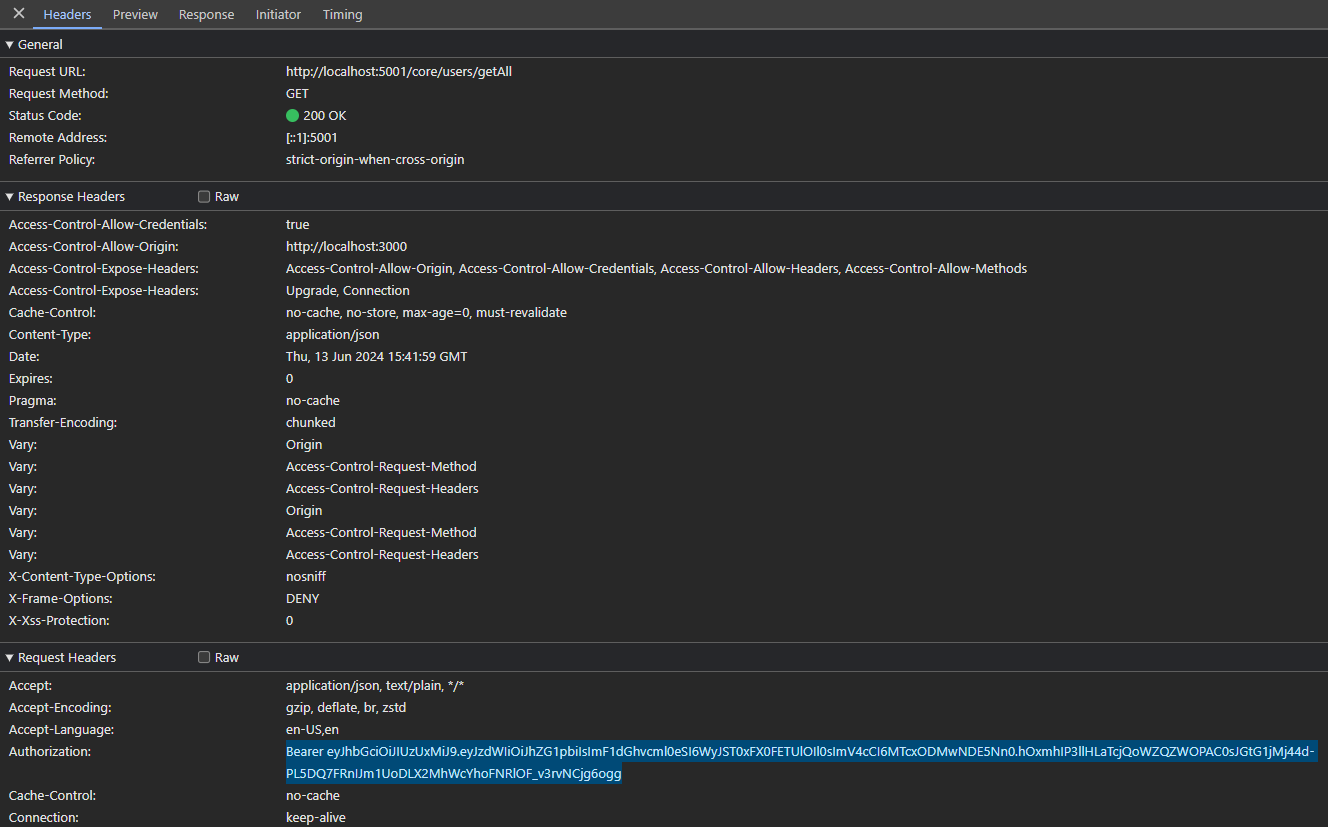
\includegraphics[width=\linewidth]{auth-token.png}
	\caption{Authorization header într-o cerere HTTP de administrator}
	\label{fig:auth-token}
 \end{figure}

\section{Funcționalitățile rolului de administrator}

Reprezentative pentru identitatea vizuală a aplicației sunt panourile de control ale administratorului, care poate accesa „Employee Directory” și „Team Manager”. Acestea se folosesc de componente reutilizabile pentru încărcarea componentei de căutare avansată și de pentru diversele formulare.

Pagina „Employee Directory” este cea încărcată default la conectarea administratorului, așa cum s-a prezentat anterior. Această pagină este compusă dintr-un tabel paginat, ce conține intrări cu toți angajații înregistrați la momentul respectiv pe platformă. Mai mult, prin intermediul unui sistem de filtrare pe bază de nume de utilizator, poziție, sau echipă, este facilitată căutarea unui angajat pentru administratori(figura \ref{fig:filter-employee}).

 \begin{figure}[H]
	\centering
 	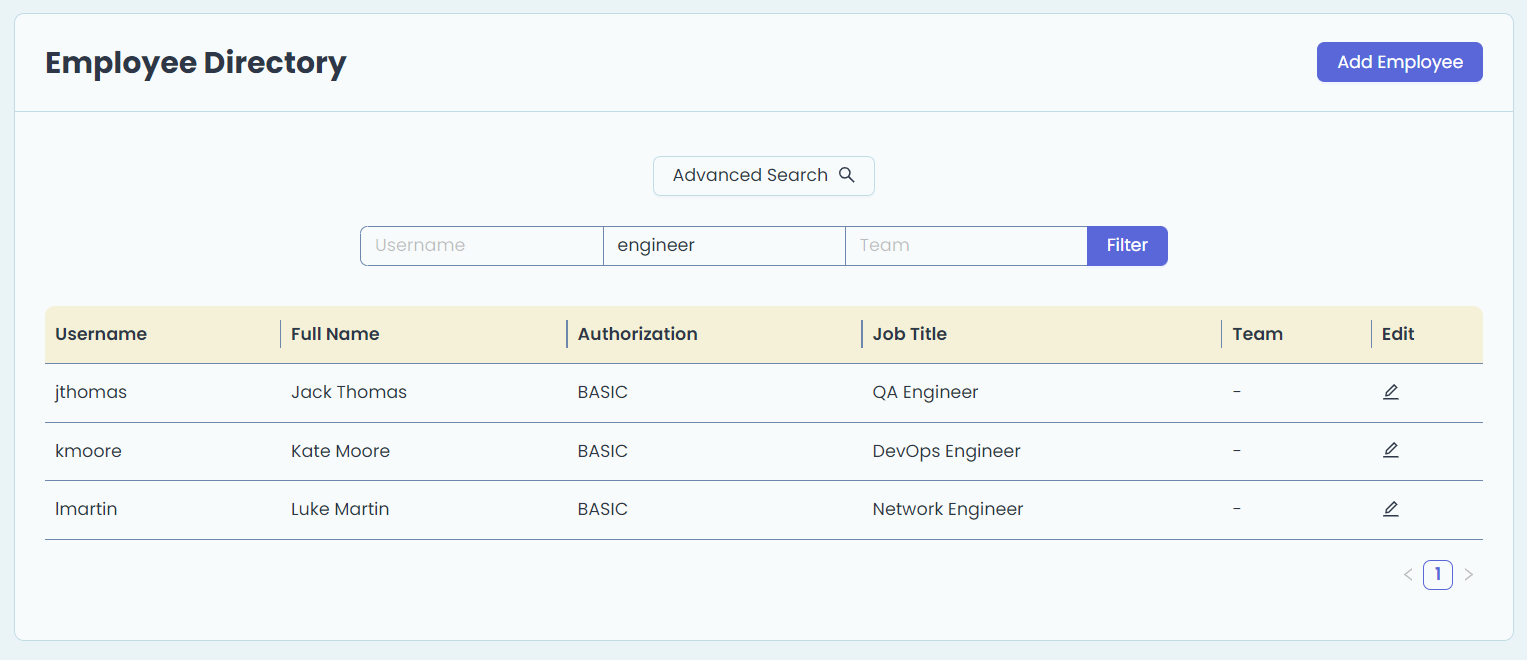
\includegraphics[width=\linewidth]{filter-employee.png}
	\caption{Rezultatul filtrării după titulatura „engineer”}
	\label{fig:filter-employee}
 \end{figure}

În plus, există funcționalități de adăugare a unui angajat nou, editarea a detaliilor privind oricare dintre angajații de pe platformă, sau ștergere a angajaților. Acestea se realizează printr-un formular generic care se randează sub două moduri, cel de creare și cel de editare(figurile \ref{fig:user-form-create} și \ref{fig:user-form-update}).

Formularul de creare a unui cont de utilizator cere introducerea tuturor datelor necesare identificării acestuia, câmpurile fiind validate înainte de trimiterea cererii către back-end.

 \begin{figure}[H]
	\centering
 	 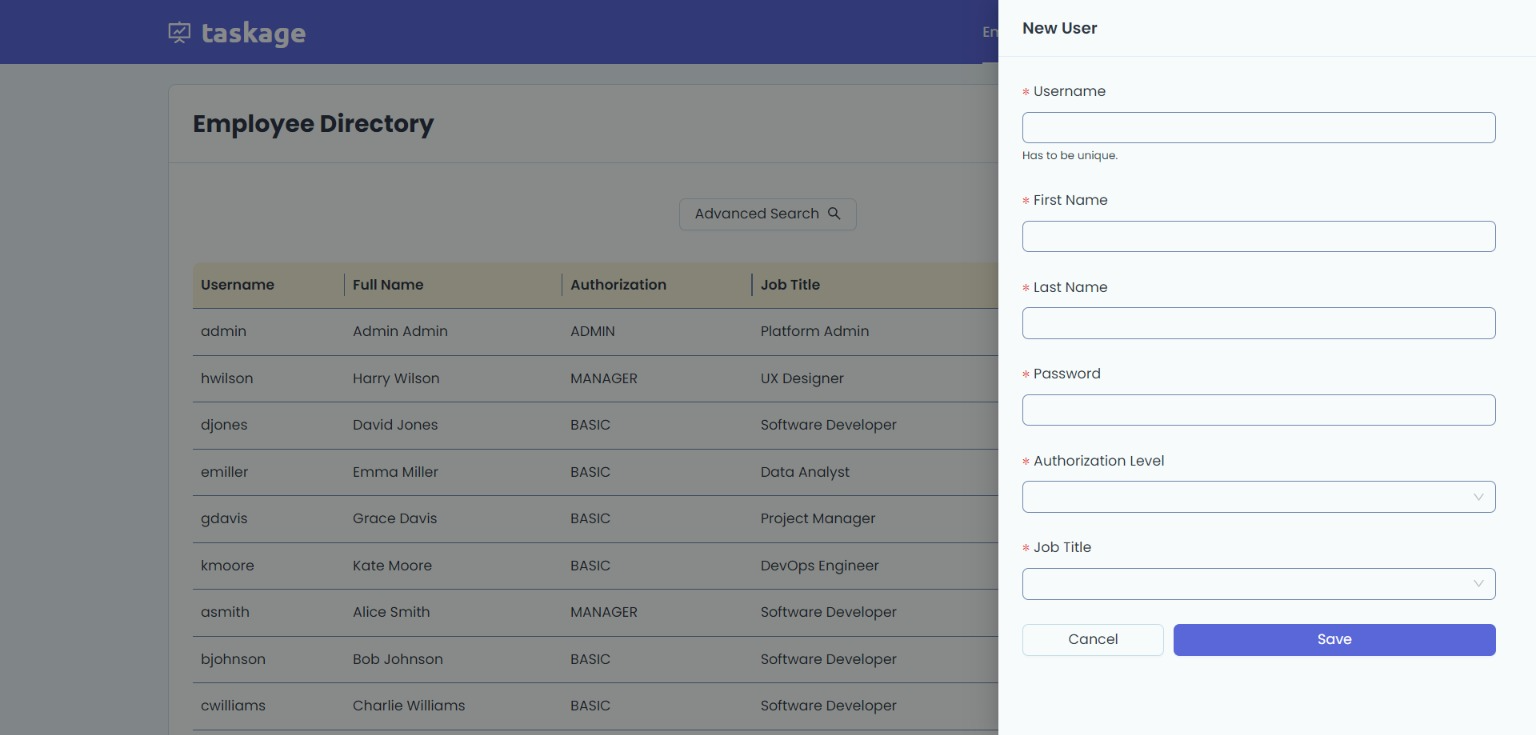
\includegraphics[width=\linewidth]{create-user-form.png}
	\caption{Formularul de creare a unui cont de utilizator}
	\label{fig:user-form-create}
 \end{figure}

Printre opțiunile oferite de caseta de selectare de Job Title se numără și posibilitatea de a salva o nouă titulatură de post, având în vedere că acestea pot varia de la organizație la organizație, în funcție de specific, și nu sunt hard-coded(figura \ref{fig:create-job-title}).

 \begin{figure}[H]
	\centering
 	 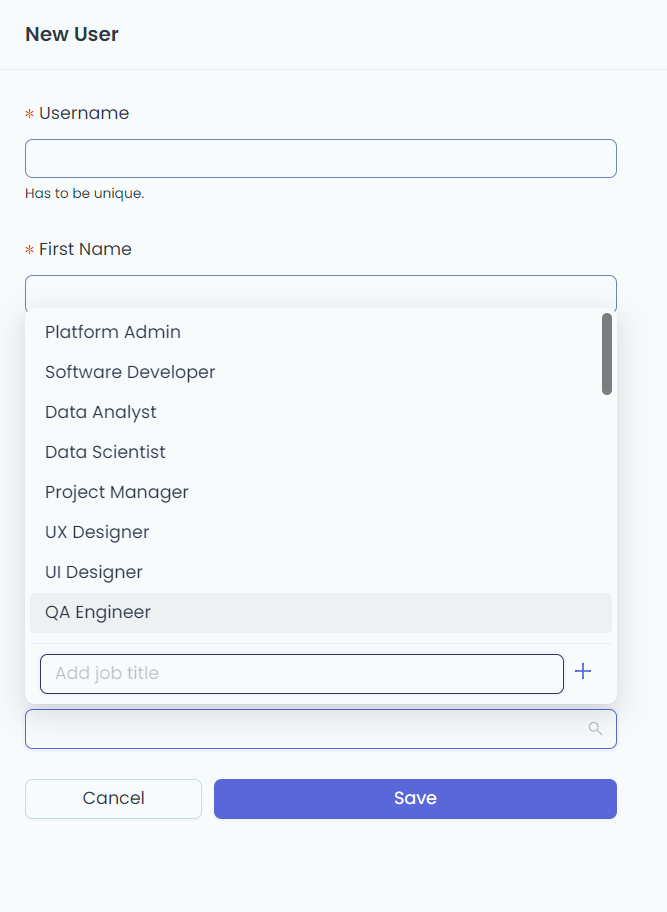
\includegraphics[width=0.5\linewidth]{create-job-title.png}
	\caption{Funcționalitatea de creare a unei noi titulaturi}
	\label{fig:create-job-title}
 \end{figure}

Formularul de actualizare este deschis prin apăsarea pictogramei în formă de creion de pe linia tabelului corespunzătoare contului ce se vrea modificat. Acesta ascunde valoarea câmpului cu parola, dar permite schimbarea ei împreună cu orice detaliu al contului. De asemenea, în colțul din dreapta sus se află butonul ce oferă posibilitatea de ștergere a contului.

 \begin{figure}[H]
	\centering
 	 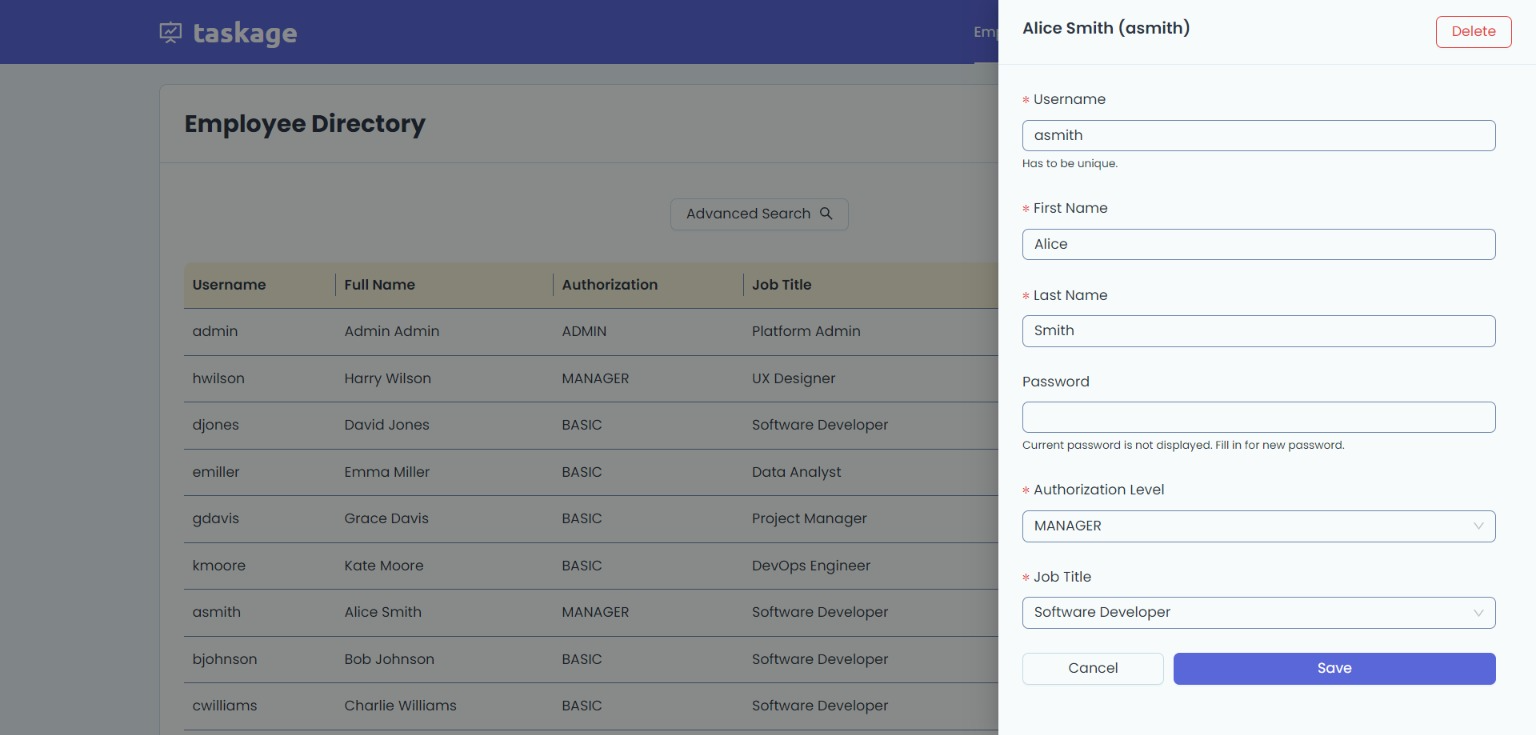
\includegraphics[width=\linewidth]{update-user-form.png}
	\caption{Formularul de actualizare a unui cont de utilizator}
	\label{fig:user-form-update}
 \end{figure}

În mod similar, administratorul are acces la „Team Manager”(figura \ref{fig:team-manager}), unde poate efectua operații similare, dar pentru echipe și componența lor. Echipele sunt prezentate sub forma unui tabel paginat care prezintă datele cele mai semnificative despre fiecare echipă, reprezentative pentru identificare: numele echipei și manager-ul(numit team lead în cadrul interfeței). Pentru vizualizarea celorlalte detalii ale echipei, este necesară apăsarea pictogramei din coloana „View” pentru echipa dorită.

 \begin{figure}[H]
	\centering
 	 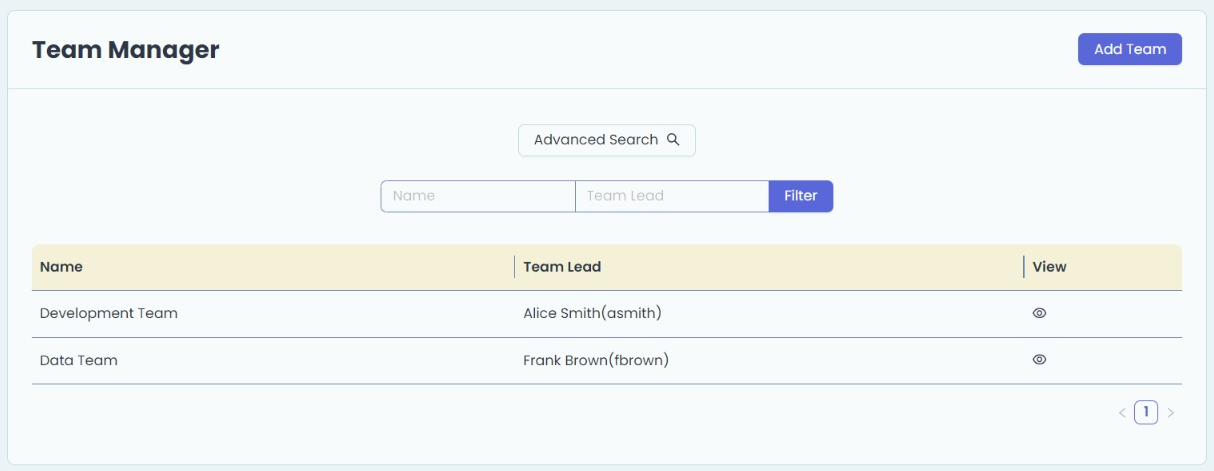
\includegraphics[width=\linewidth]{team-manager-1.png}
	\caption{Team Manager}
	\label{fig:team-manager}
 \end{figure}

Odată cu apăsarea acestei pictograme, se va deschide un side panel cu informațiile complete(figura \ref{fig:team-panel-read}). Acesta este, la fel ca cel de creare a unui cont de utilizator, generic, în sensul în care se randează, atât sub forma de vizualizare, cât și sub alte două moduri: creare și editare(figura \ref{fig:team-panel}). Formularele au restricții specifice. De exemplu, un utilizator poate fi membru al unei singure echipe, iar numele echipei trebuie să fie unic.

 \begin{figure}[H]
	\centering
	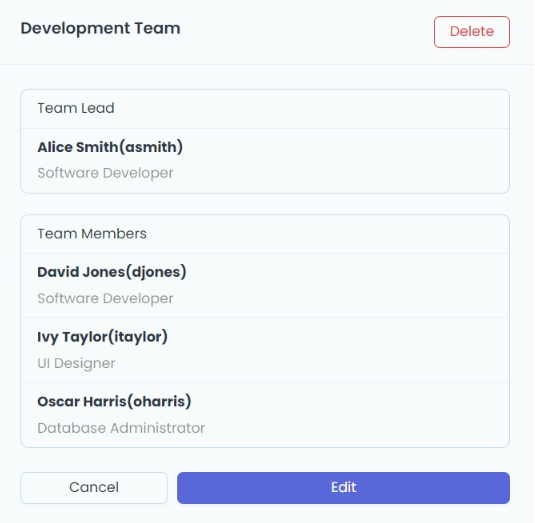
\includegraphics[width=0.5\linewidth]{team-read-1.png}
	\caption{Side panel de echipă sub forma de vizualizare}
	\label{fig:team-panel-read}
 \end{figure}

 \begin{figure}[H]
 	 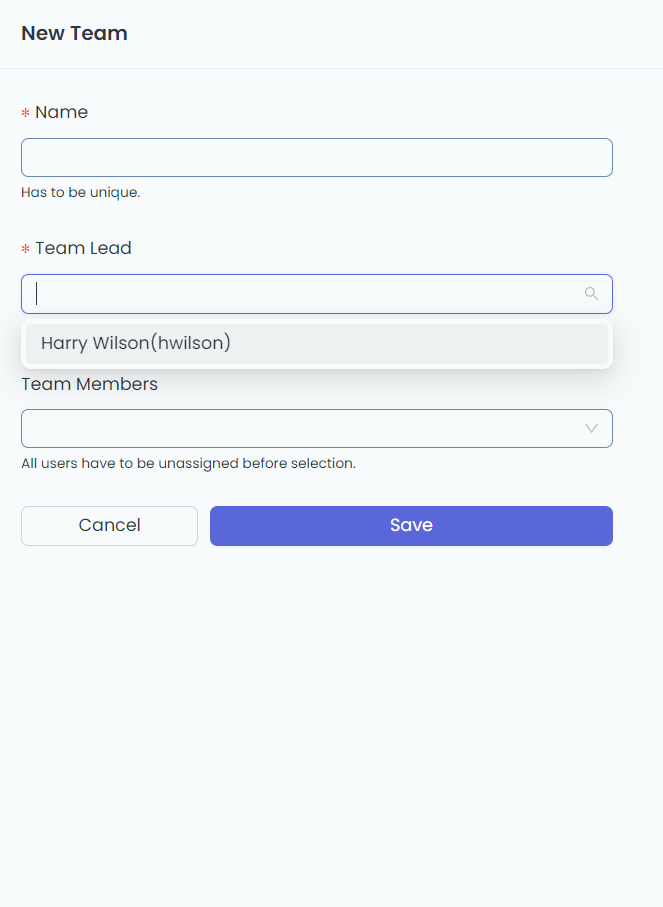
\includegraphics[width=0.5\linewidth]{team-create-1.png}
	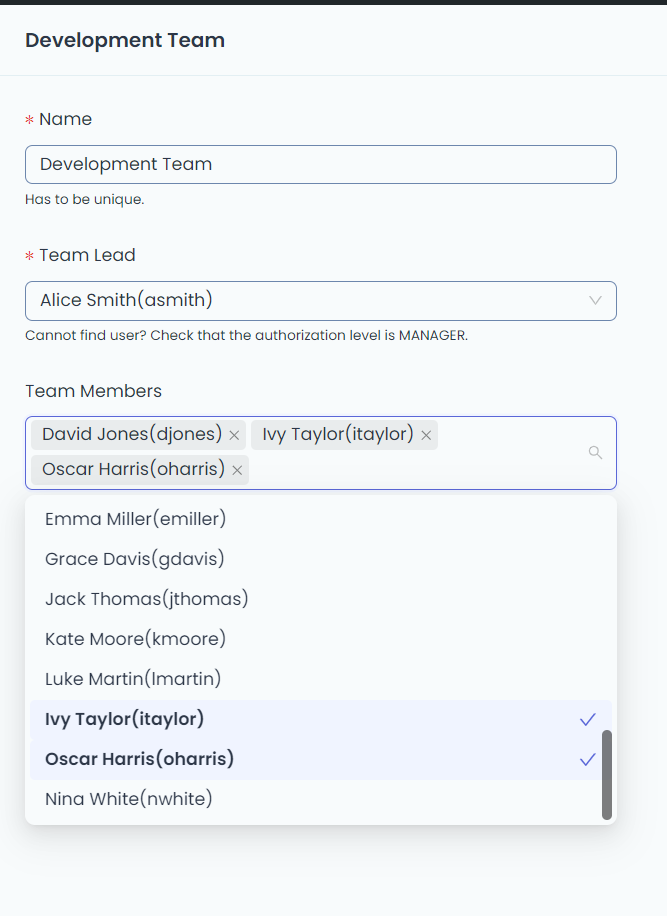
\includegraphics[width=0.5\linewidth]{team-update-1.png}
	\caption{Side panel de echipă sub formele: creare, editare}
	\label{fig:team-panel}
 \end{figure}

De asemenea, administratorul dispune de o pagina numită „My Metrics”(figura \ref{fig:my-metrics}) unde poate vizualiza componenta „Admin Dashboard”.

 \begin{figure}[H]
	\centering
 	 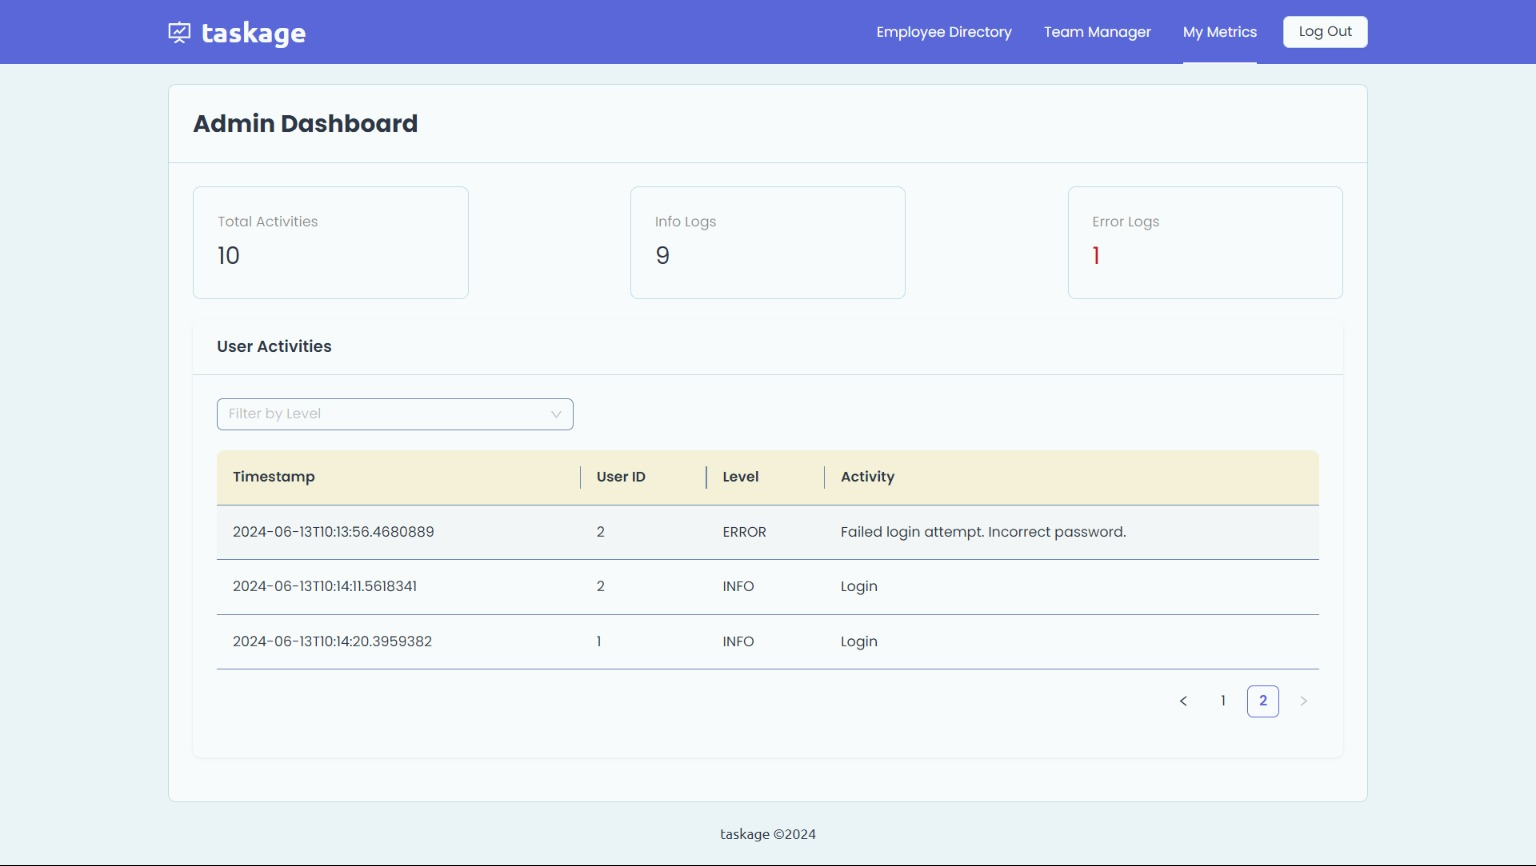
\includegraphics[width=\linewidth]{my-metrics.png}
	\caption{Pagina „My Metrics”}
	\label{fig:my-metrics}
 \end{figure}

De pe această pagină, administratorul află informații despre utilizarea platformei, poate urmări activitatea utilizatorilor și eventualele erori întâmpinate în cadrul unui tabel cu informații despre când, cine și ce activitate a declanșat, primind o imagine de ansamblu asupra gradului de utilizare și eficiență al platformei.

\section{Funcționalitățile rolului de manager}

Utilizatorul cu rol de manager are la dispoziție două componente principale: „Sprint Dashboard” și „Team Details”. După autentificare, este redirecționat către „Sprint Dashboard”, adică panoul de sprint(figura \ref{fig:sprint-dashboard}) al propriei echipe, care funcționează ca un intrument de gestiune a sarcinilor de lucru și a sprinturilor.

Aici, utilizatorul poate vizualiza toate sarcinile de lucru încadrate în sprintul curent, grupate după statusul lor: To Do, In Progress și Done. În cadrul acestei interfețe sunt afișate informațiile esențiale unui task, și anume titlu, prioritate, membru al echipei asignat și progres.

 \begin{figure}[H]
	\centering
 	 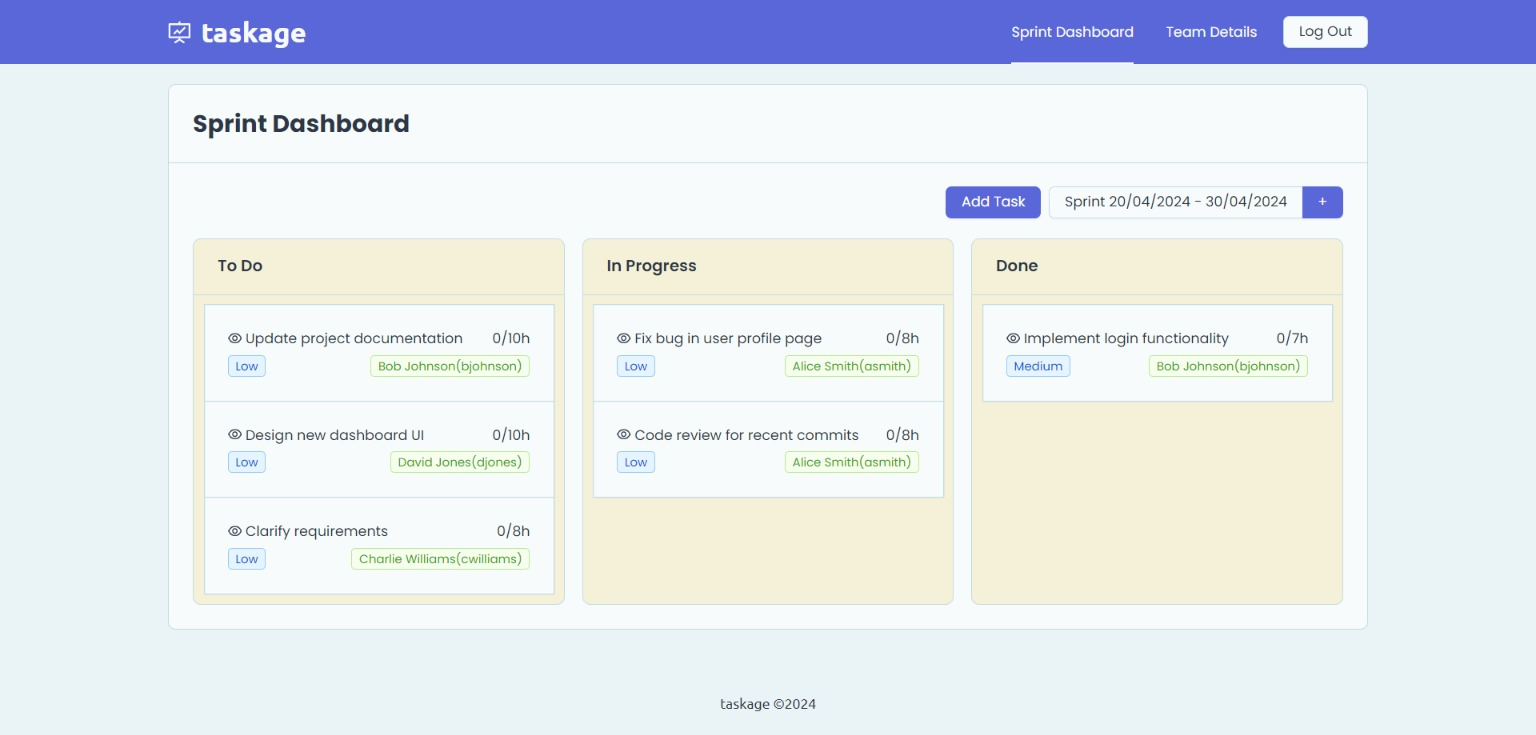
\includegraphics[width=\linewidth]{sprint-dashboard.png}
	\caption{„Sprint Dashboard” - panoul de sprint}
	\label{fig:sprint-dashboard}
 \end{figure}

Pentru vizualizarea celorlalte informații referitoare la task(puncte de efort, tip de task, descriere), manager-ul trebuie să apese pictograma de langă titlul task-ului dorit, care va deschide un side panel ca cel din figura \ref{fig:task-view}, care poate trece în modul de editare prin apăsarea butonului „Edit”.

 \begin{figure}[H]
	\centering
 	 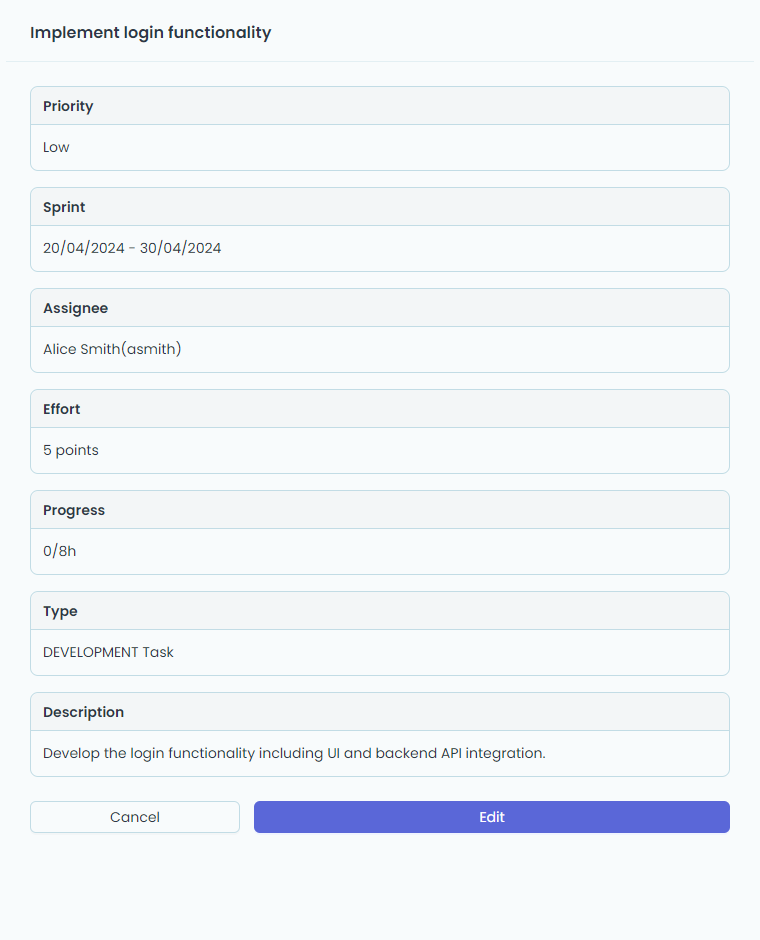
\includegraphics[width=0.5\linewidth]{task-view.png}
	\caption{Side panel cu detaliile sarcinii de lucru}
	\label{fig:task-view}
 \end{figure}

Pentru crearea unui nou task, utilizatorul apasă butonul „Add Task” de pe aceeași pagină, care va deschide într-un side panel formularul din figura \ref{fig:task-create}.

 \begin{figure}[H]
	\centering
 	 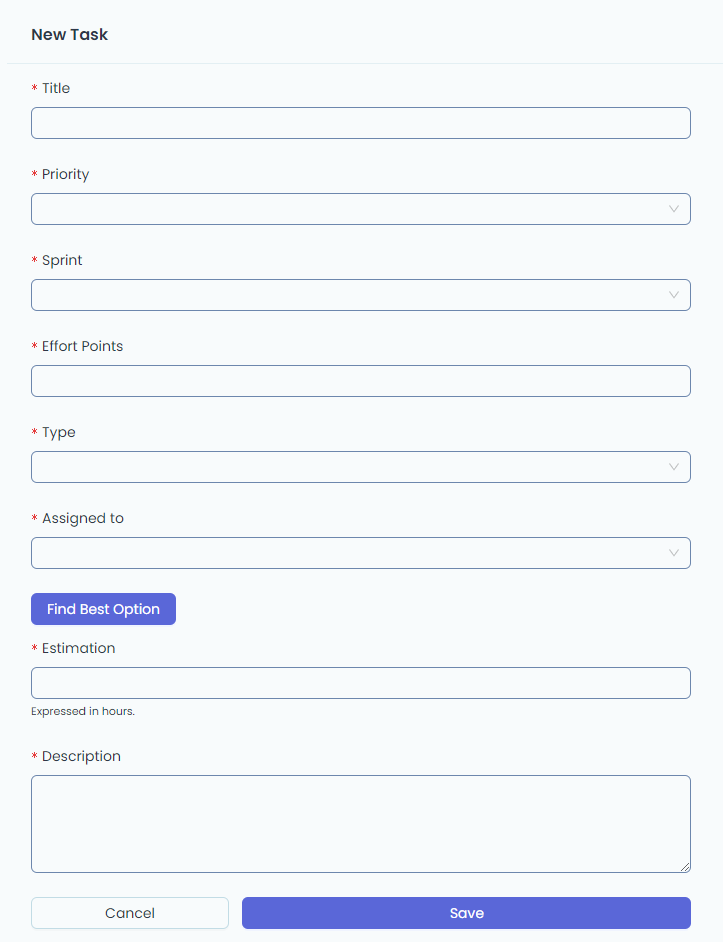
\includegraphics[width=0.5\linewidth]{task-create.png}
	\caption{Formularul de creare a unei sarcini de lucru}
	\label{fig:task-create}
 \end{figure}

Funcționalitatea implementată de Taskage-Helper, descrisă în secțiunea 4.6, este utilizată în cadrul acestui formular. Butonul „Find Best Option” declanșează generarea unei sugestii, însă pentru calculele de similaritate este nevoie de completarea unor câmpuri esențiale: prioritate, sprint, puncte de efort, tip de sarcină de lucru. În cazul în care aceste câmpuri nu sunt completate, butonul va afișa un mesaj care indică că este nevoie de completarea lor(figura \ref{fig:task-create-disabled}).

 \begin{figure}[H]
	\centering
 	 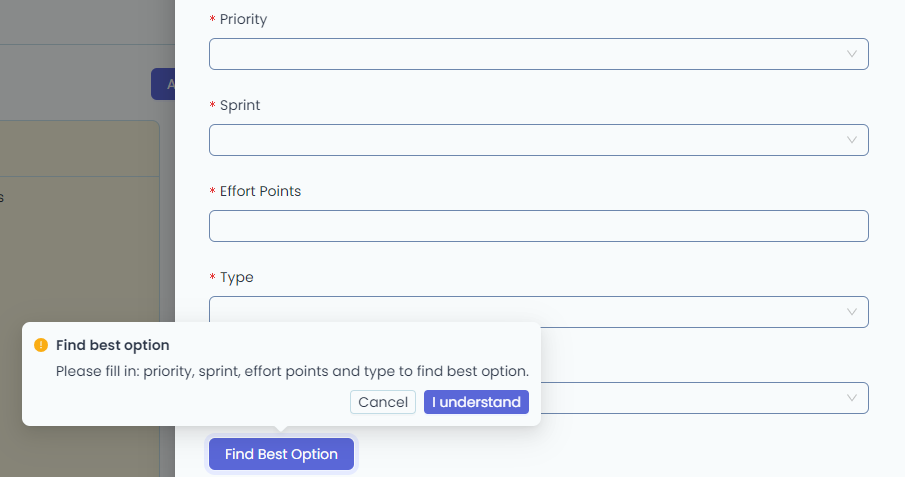
\includegraphics[width=0.7\linewidth]{task-create-disabled.png}
	\caption{Răspunsul „Find Best Option” atunci când nu sunt completate câmpurile necesare}
	\label{fig:task-create-disabled}
 \end{figure}

Dacă aceste câmpuri sunt completate, algoritmul va genera sugestia și o va prezenta cu opțiunile de acceptare, care va selecta automat sugestia pentru câmpul „Assigned to”, sau respingere, pentru eventuală selecție manuală(figura \ref{fig:task-create-enabled}).

 \begin{figure}[H]
	\centering
 	 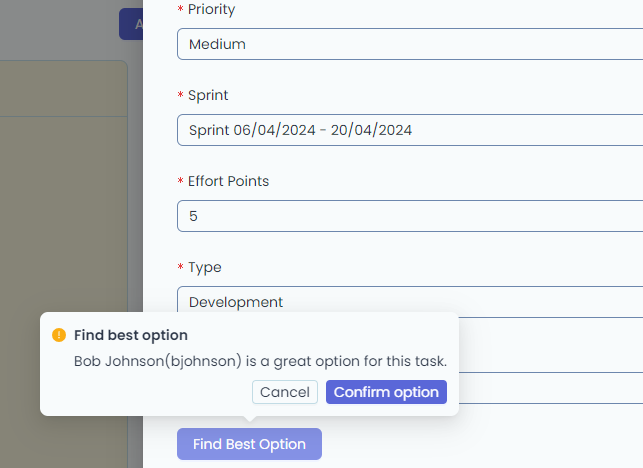
\includegraphics[width=0.7\linewidth]{task-create-enabled.png}
	\caption{Răspunsul „Find Best Option” atunci când sunt completate câmpurile necesare}
	\label{fig:task-create-enabled}
 \end{figure}

De asemenea, utilizatorul poate gestiona sprinturile cu ajutorul setului de componente din figura \ref{fig:new-sprint}. Cu ajutorul primei componente, acesta poate selecta sprint-ul pe care dorește să în vizualizeze cu ajutorul unui meniu drop-down sau poate crea un sprint nou apăsând pe butonul „+”, ce deschide a doua componentă ilustrată, un modal. Mai departe, trebuie să selecteze data de început și data de final a sprintului. Datele pe care le are la dispoziție pentru crearea sprintului sunt datele care urmează ultimului sprint creat, fără să existe posibilitatea de a adăuga sprinturi în trecut, așa cum se poate observa în a treia captură de ecran a figurii, unde parte din calendar este dezactivată.

 \begin{figure}[H]
	\centering
	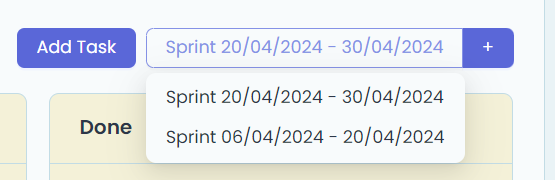
\includegraphics[width=0.5\linewidth]{sprint-dropdown.png}
 	 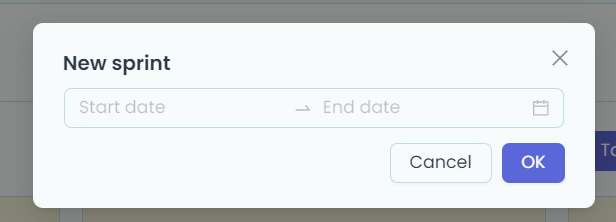
\includegraphics[width=0.5\linewidth]{new-sprint-form.png}
	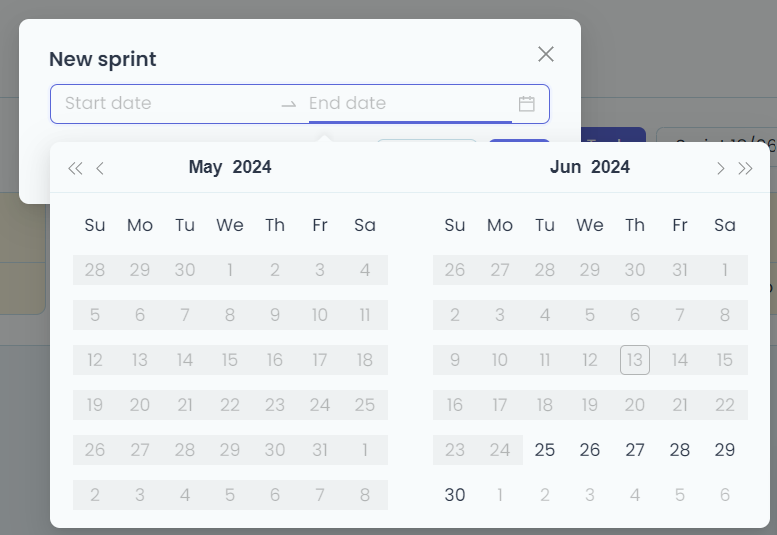
\includegraphics[width=0.5\linewidth]{new-sprint-calendar.png}
	\caption{Componentele pentru gestionarea sprinturilor}
	\label{fig:new-sprint}
 \end{figure}

Tot ce ține de panoul cu sarcini de lucru este actualizat în timp real cu ajutorul WebSockets, mecanism prezentat în secțiunea 4.5. În zona „Network” a Developer Tools din browser, putem vizualiza datele primite prin WebSocket. De exemplu, pentru acțiunea „UPDATE”(figura \ref{fig:task-ws}), sarcina de lucru actualizată se va schimba în timp real pentru toți utilizatorii prezenți pe pagina panoului de task-uri.

 \begin{figure}[H]
	\centering
 	 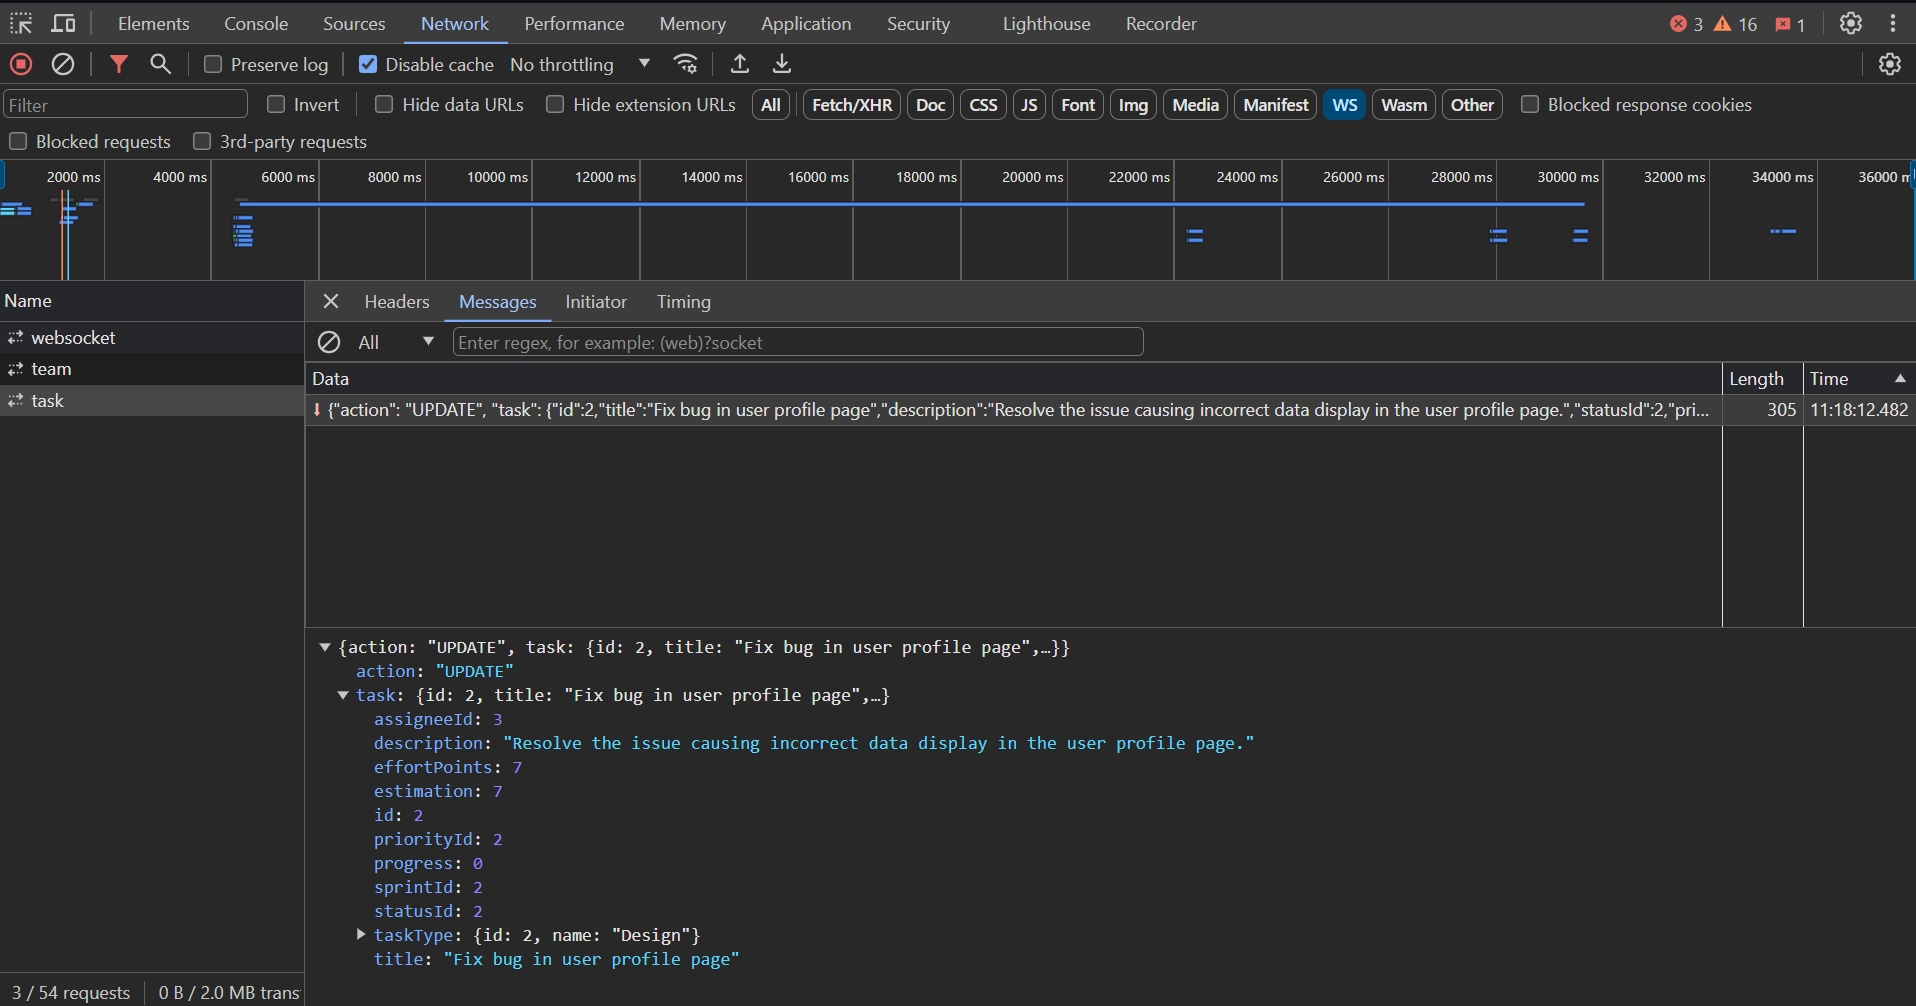
\includegraphics[width=\linewidth]{task-ws.png}
	\caption{Acțiunea „UPDATE” primită prin WebSocket}
	\label{fig:task-ws}
 \end{figure}

Rezultatul acestui mesaj primit prin WebSocket reiese din faptul că, mai mulți utilizatori, sau chiar și mai multe instanțe de browser ale aceluiași utilizator vor fi mereu sincronizate din punct de vedere al datelor afișate(figurile \ref{fig:ws-sync-1} și \ref{fig:ws-sync-2}).

 \begin{figure}[H]
	\centering
 	 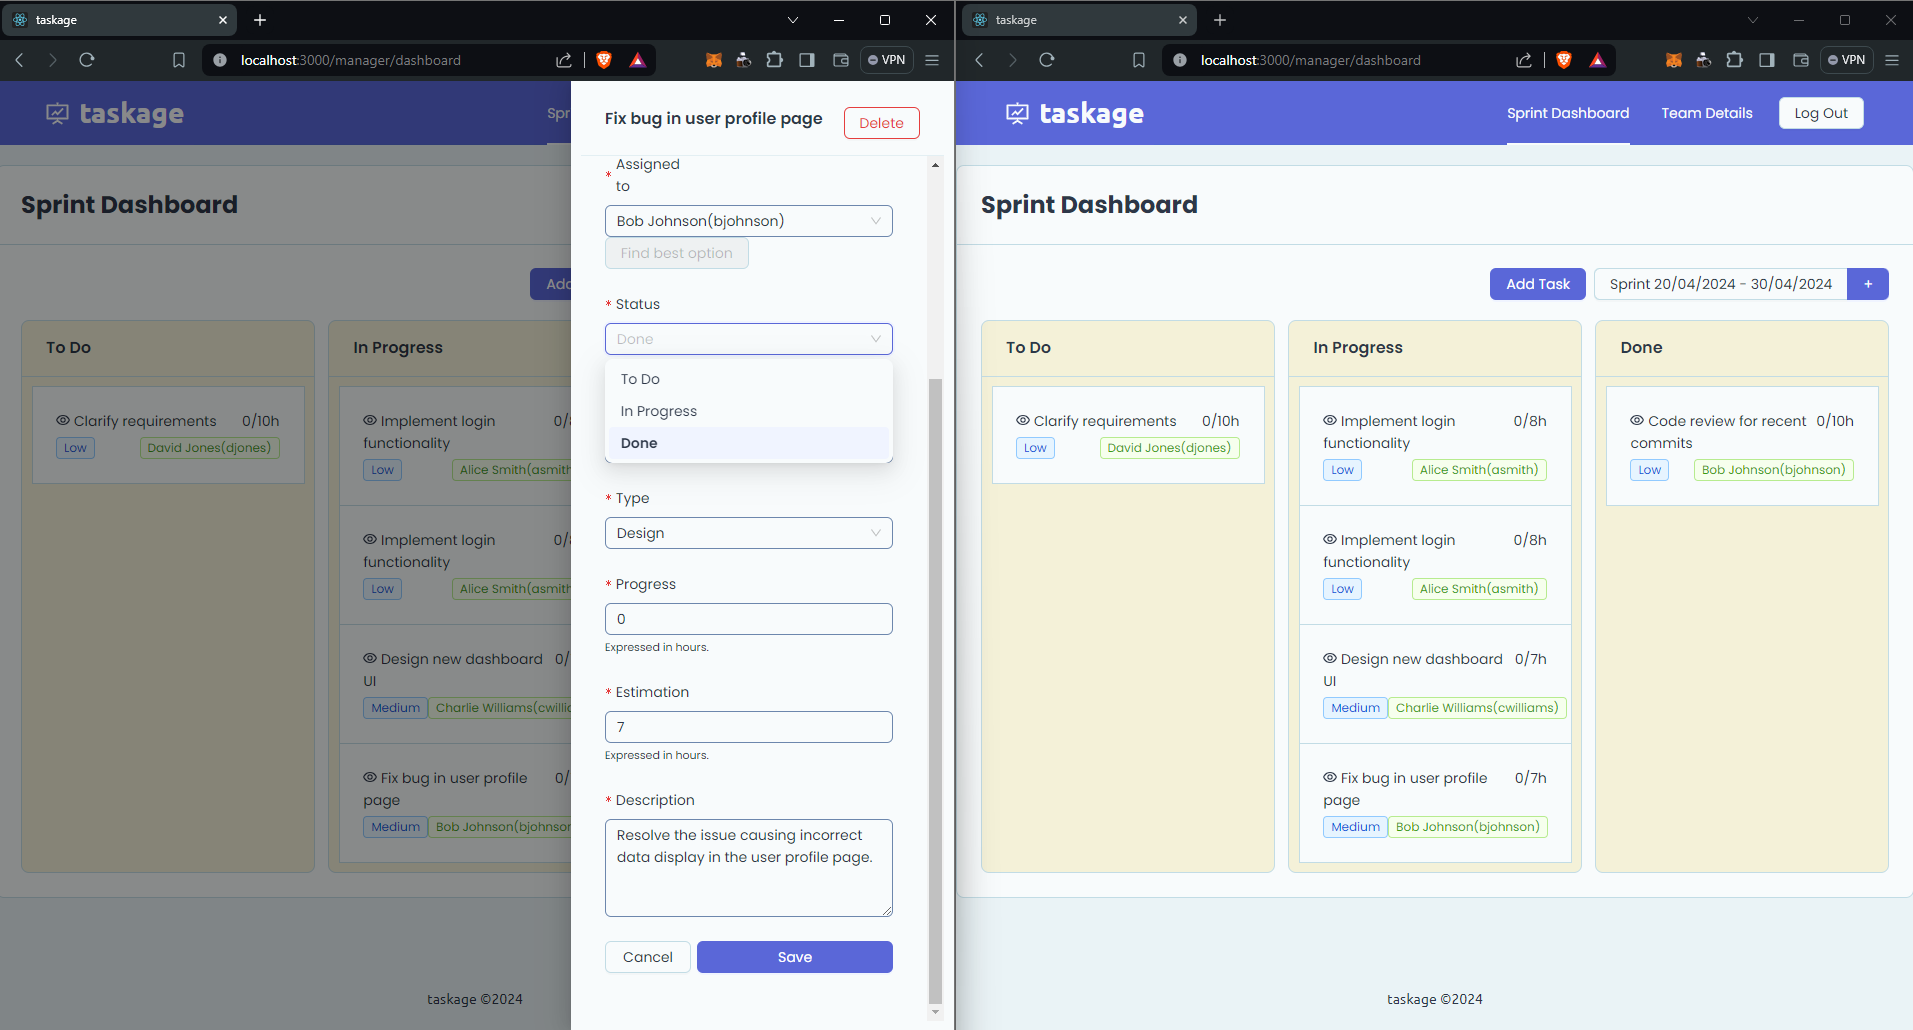
\includegraphics[width=\linewidth]{before-save.png}
	\caption{Acțiunea de actualizare sincronizată}
	\label{fig:ws-sync-1}
 \end{figure}

 \begin{figure}[H]
	\centering
	 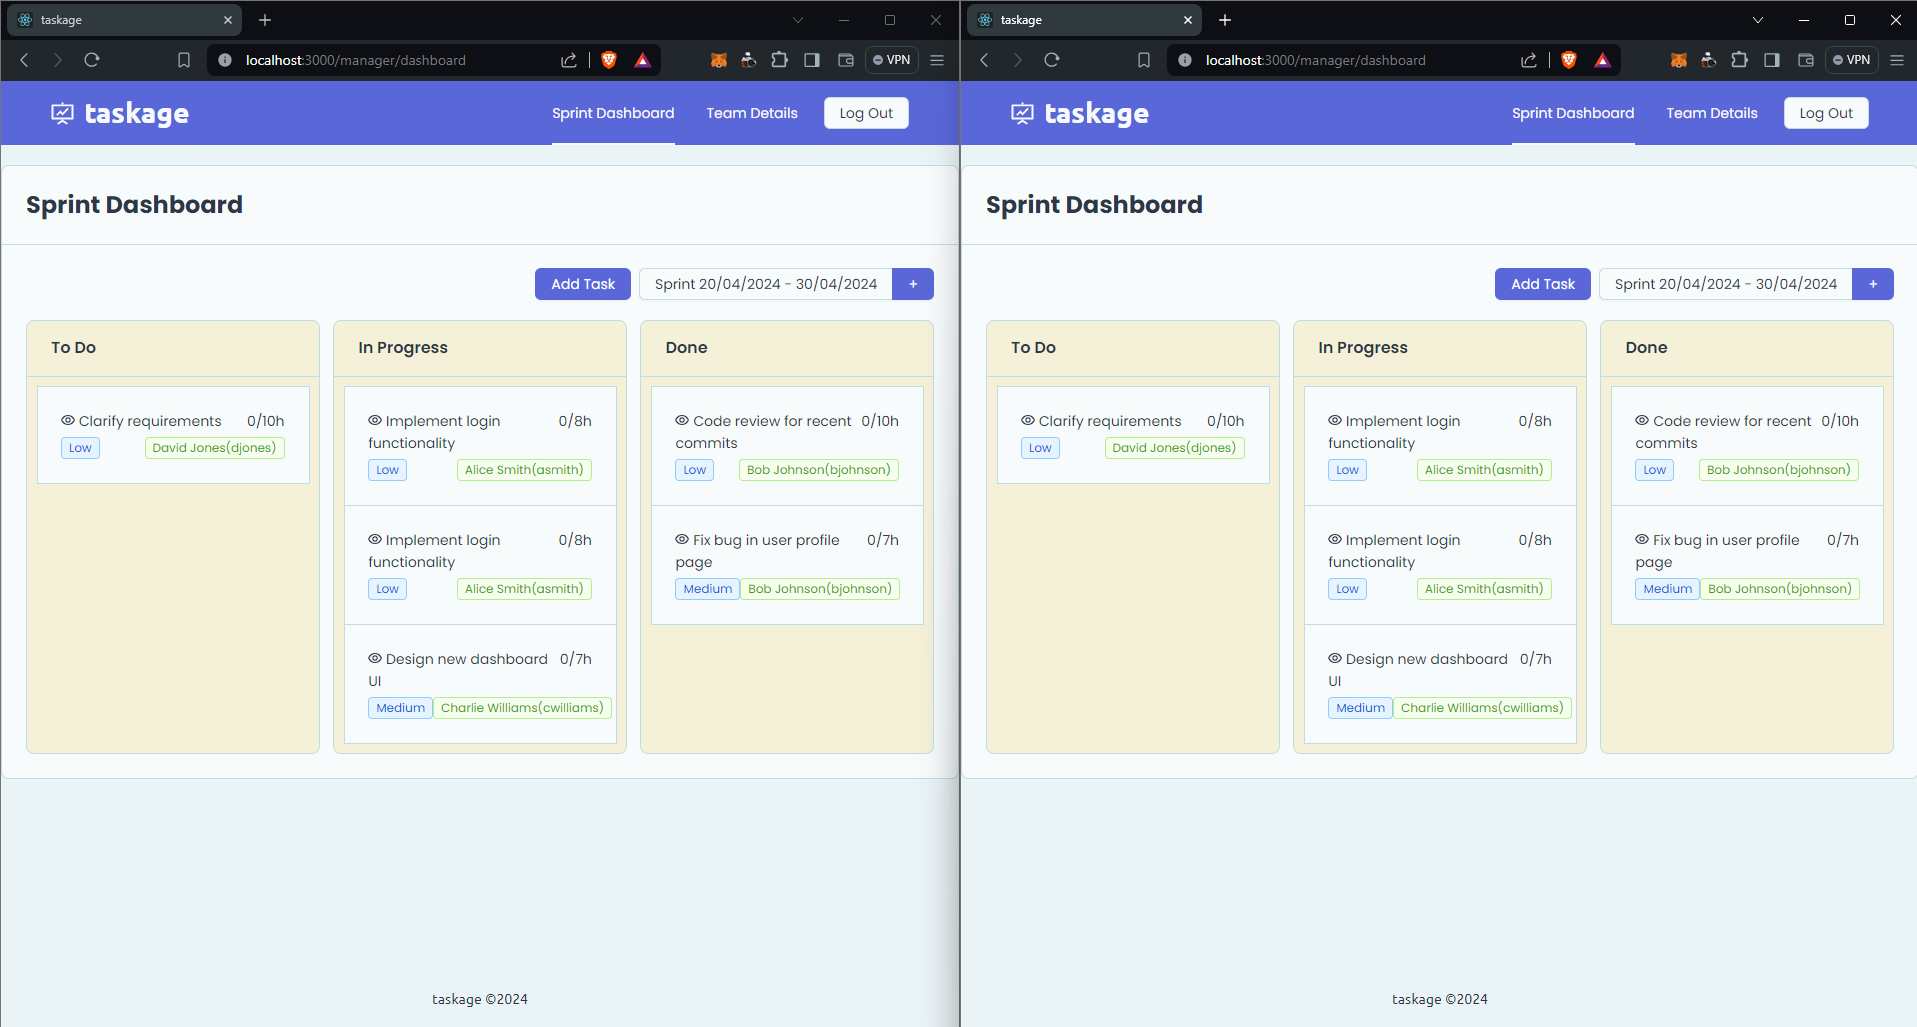
\includegraphics[width=\linewidth]{after-save.png}
	\caption{Rezultatul acțiunii de actualizare sincronizată}
	\label{fig:ws-sync-2}
 \end{figure}

Cealaltă rută, „Team Details”, oferă detalii legat de capacitatea membrilor echipei, calculând raportul dintre numărul total de ore al sprintului și estimările sarcinilor asignate fiecărui membru al echipei(figura \ref{fig:team-details}). Aceste statistici sunt exprimate per sprint, care poate fi selectat dintr-un drop-down reutilizat din componenta „Sprint Dashboard”. Rolul lor este de a facilita alegerea în cazul asignării manuale, reprezând într-un mod de înțeles disponibilitatea fiecărui membru al echipei.

 \begin{figure}[H]
	\centering
 	 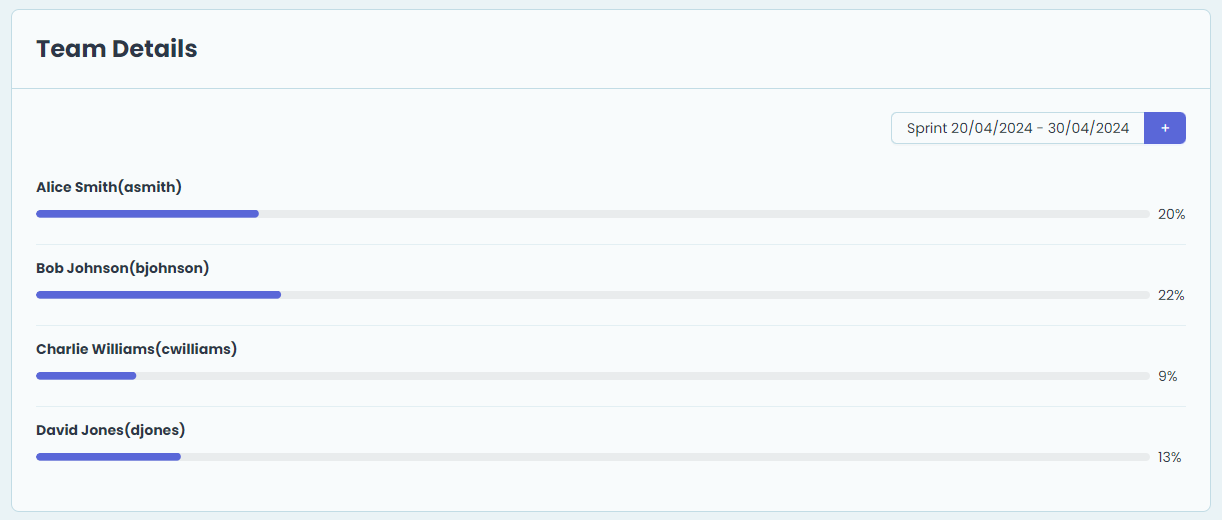
\includegraphics[width=\linewidth]{team-details.png}
	\caption{Statisticile capacității membrilor echipei}
	\label{fig:team-details}
 \end{figure}

\section{Funcționalitățile rolului de membru de echipă}

Utilizatorii simpli dispun de funcționalități asemănătoare managerilor, așa că urmează să expun doar capabilitățile diferite.

Asemănător rolului de manager, după autentificare, utilizatorul simplu este redirecționat către Sprint Dashboard, însă aici își poate vizualiza numai atribuțiile personale(figura \ref{fig:basic-sprint-dashboard}).

 \begin{figure}[H]
	\centering
 	 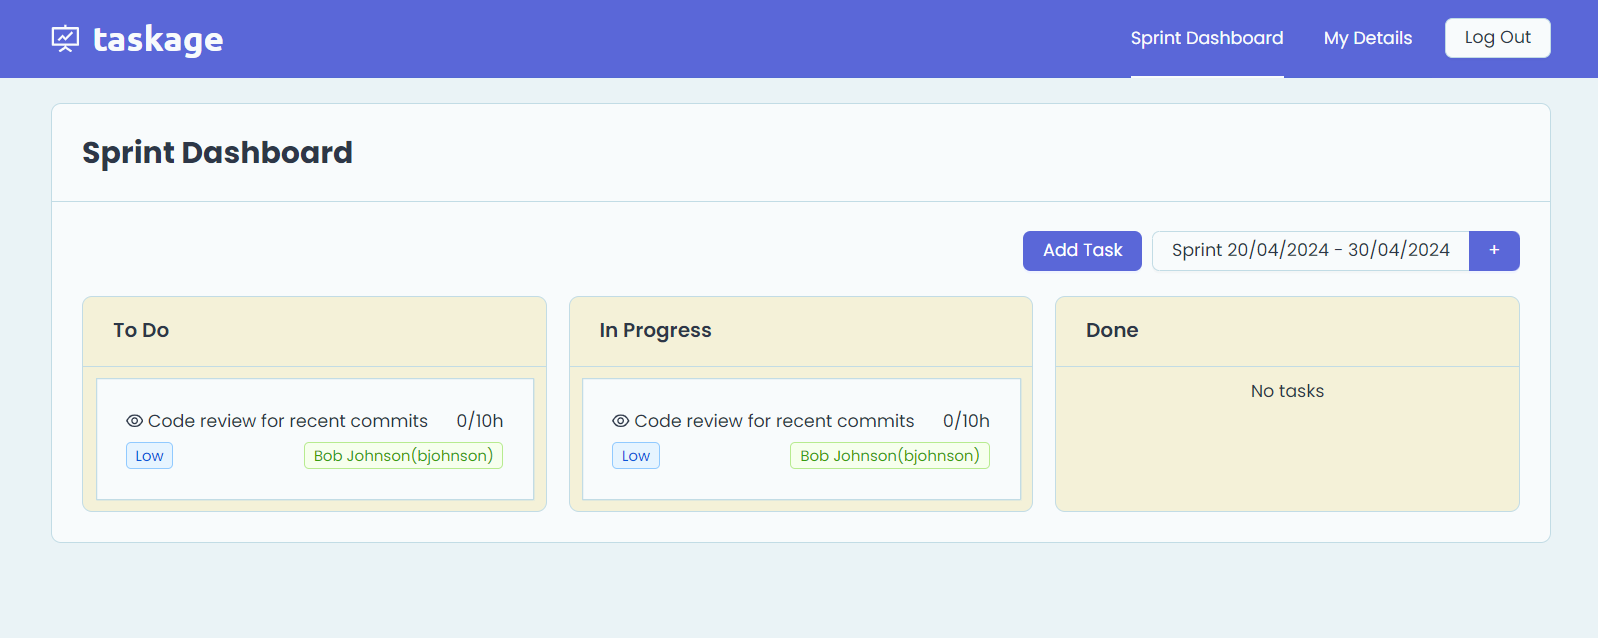
\includegraphics[width=\linewidth]{basic-sprint-dashboard.png}
	\caption{„Sprint Dashboard” din perspectiva unui simplu membru de echipă}
	\label{fig:basic-sprint-dashboard}
 \end{figure}

Acesta primește un nou tip de notificări, prin care este informat atunci când managerul său i-a asignat un nou task(figura \ref{fig:new-task-toast}), ca răspuns la mesajul specific primit prin sistemul WebSocket descris anterior, în secțiunea 4.5.

 \begin{figure}[H]
	\centering
 	 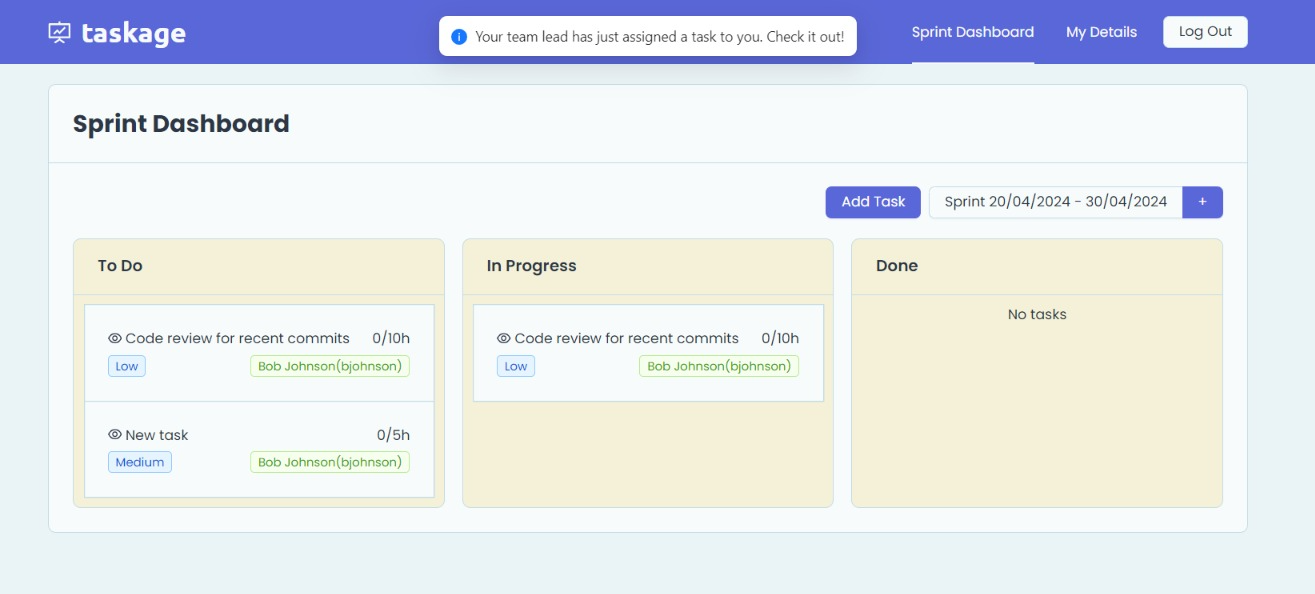
\includegraphics[width=\linewidth]{new-task-toast.png}
	\caption{„New task” în Sprint Dashboard și notificarea aferentă}
	\label{fig:new-task-toast}
 \end{figure}

O altă diferență este vizibilă pe pagina „My details”, care este o variantă personalizată a „Team Details”. Aici, utilizatorul poate să vadă, măsurată, performanța sa pe parcursul ultimelor cinci sprinturi și capacitatea sprintului curent, raportată la sarcinile de lucru care i-au fost asignate și estimările lor(figura \ref{fig:my-stats}).

 \begin{figure}[H]
	\centering
 	 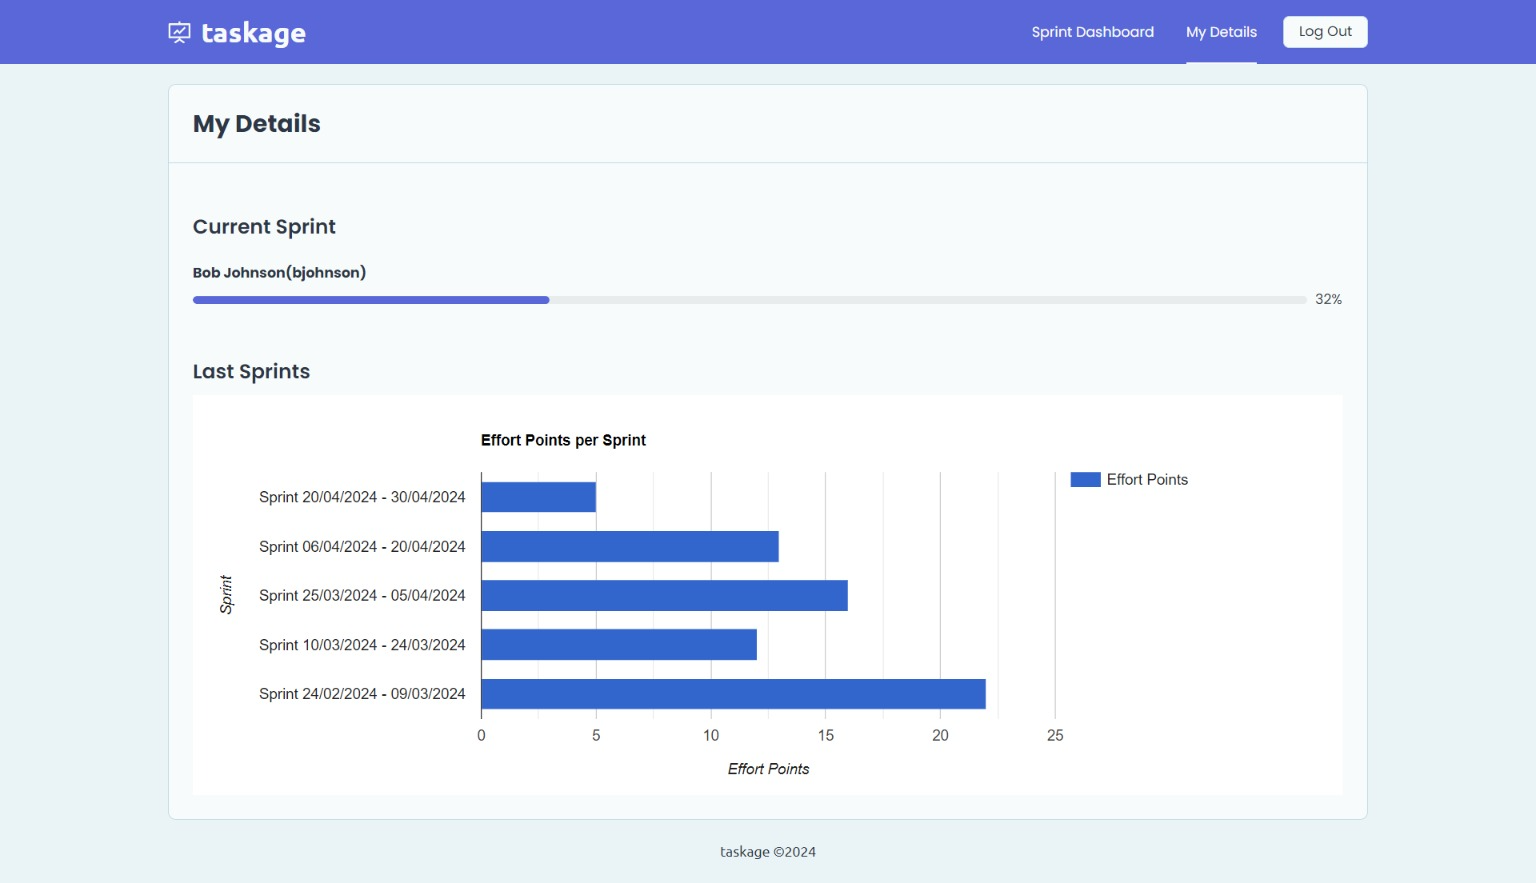
\includegraphics[width=\linewidth]{my-stats.png}
	\caption{Pagina de statistici a unui utilizator simplu}
	\label{fig:my-stats}
 \end{figure}
